\section{SCGRA Overlay Based FPGA Accelerator Customization} \label{sec:customization-framework}
Application-specific customization provides unique opportunity to improve 
the energy and performance of the resulting accelerators. However, 
taking the system as a black box and exhaustively searching all the 
possible configurations can be inefficient and slow. In this work, by taking advantage 
of the regularity of the SCGRA overlay based FPGA accelerator, we 
can reduce the complex customization problem to a much simpler sub design space exploration (DSE)
together with a simplified search problem and optimized application-specific 
nested loop accelerator can be produced efficiently.

\subsection{Customization problem formulation}
In this section, we will formalize the customization problem of the nested loop acceleration on an
SCGRA overlay based FPGA accelerator. Various design constraints including energy consumption and
hardware resource overhead can be used while hardware overhead is taken as an example here.

\begin{table}[tb]
    \begin{threeparttable}
\scriptsize
\centering
\caption{Design Parameters of Nested Loop Acceleration\label{tab:parameter-list}}{
\begin{tabular}{l|l|l}
\hline
\multicolumn{2}{l|}{Design Parameters} & Denotation \\ \hline
\multirow{2}{*}{\tabincell{l}{Nested Loop \\ Compilation}} & Loop Unrolling Factor & $\bm{u}=(u_0,u_1, ...)$  \\ \cline{2-3} 
                                                           & Grouping Factor & $\bm{g}=(g_0, g_1, ...)$ \\ \hline
\multirow{11}{*}{\tabincell{l}{Overlay \\ Configuration}}  & SCGRA Topology  & Null, 2D Torus \\ \cline{2-3} 
                                                          & SCGRA Size  & $r\times c$ \\ \cline{2-3}
                                                          & Instruction Mem & $imD \times imW$ \\ \cline{2-3}
                                                          & Data Mem & $dmD \times dmW$ \\ \cline{2-3}
                                                          & Input Buffer & $ibD \times ibW$ \\ \cline{2-3}
                                                          & Output Buffer & $obD \times obW$ \\ \cline{2-3}
                                                          & Input Address Buffer & $iabD \times iabW$ \\ \cline{2-3}
                                                          & Output Address Buffer & $oabD \times oabW$ \\ \cline{2-3}
                                                          & Operation Set & Null, fixed \\ \cline{2-3}
                                                          & Implementation Frequency & $f$, fixed \\ \hline
                                                          & Pipeline Depth & Null, fixed \\ \hline
\end{tabular}
\begin{tablenotes}
    \small
\item Null means there is no denotation for that parameter.
\end{tablenotes}
}
\end{threeparttable}
\end{table}

Suppose $\bm{\Psi}$ represents the overall nested loop acceleration design 
space. $\bm{C} \in \bm{\Psi}$ represents a possible configuration in 
the design space and it includes a number of design parameters as  
listed in \tabref{tab:parameter-list}. Assume that the loop to be accelerated 
has $n$ nested levels and loop count can be denoted as $l=(l_1, l_2, ..., l_n)$.
$R=(R_1, R_2, R_3, R_4)$ stands for the FPGA resource (i.e. BRAM, DSP, LUT and FF) 
that are available on a target FPGA and $Overhead(\bm{C}, i)$ denotes the 
four different types of FPGA resource overhead. $In(\bm{g})$ and $Out(\bm{g})$ 
stand for the amount of input and output of a group. Similarly, $In(\bm{u})$ 
and $Out(\bm{u})$ stand for the amount of input and output of a DFG. 
$DFGCompuTime(\bm{C})$ represents the number of cycles needed to 
complete the DFG computation. $\alpha_i$ and $\beta_i$ are constant 
coefficients depending on target platform where $i=(1,2,...)$. With these denotations, 
the customization problem targeting minimum energy consumption can be formulated 
as follows:

Minimize 
\begin{equation} \label{eq:runtime}
    \scriptsize
    RunTime(\bm{C})=CompuTime(\bm{C})+CommuTime(\bm{C})
\end{equation}
subject to
\begin{equation} \label{eq:constraints}
    \scriptsize
    \begin{split}
        &Overhead(\bm{C}, i) \leq R_i, i=1,2,3,4 \\
        &In(g) \leq ibD \\
        &Out(g) \leq obD \\
        &DFGCompuTime(\bm{C}) \leq imD \\
        &\displaystyle \prod_{i=1}^{n} \frac{g_i}{u_i} \times In(u) \leq iabD \\
        &\displaystyle \prod_{i=1}^{n} \frac{g_i}{u_i} \times Out(u) \leq oabD
    \end{split}
\end{equation}

$RunTime(\bm{C})$ represents the number of cycles needed to compute the loop on 
the CPU-FPGA system. It consists of both the time consumed for computing on FPGA and 
communication between FPGA and host CPU, and it can be calculated using \eqnref{eq:runtime}.

Since the unrolled part of the loop will be translated to 
DFG and then scheduled to the SCGRA overlay. Thus the DFG computation time 
is essentially a function of $\mathbf{u}$, $r$ and $c$, and it can also be 
denoted by $DFGCompuTime(\mathbf{u},r,c)$.
The nested loop is computed by repeating the same DFG execution, and the 
nested loop computation can be calculated using \eqnref{eq:loopexetime}.
\begin{equation} \label{eq:loopexetime}
    \scriptsize
    CompuTime(\bm{C})=\displaystyle \prod_{i=1}^{n} \frac{l_i}{u_i} \times DFGCompuTime(\mathbf{u},r,c)
\end{equation}

DMA is typically used for the bulk data transmission. Communication cost per 
data can be modeled with a piecewise linear function and thus DMA latency can be 
calculated using $DMA(x)$ where $x$ represents the amount of DMA transmission. The communication
time of the whole nested loop can be calculated by \eqnref{eq:commu}.
\begin{equation} \label{eq:commu}
    \scriptsize
    CommuTime(\bm{C})=\displaystyle \prod_{i=1}^{n} \frac{l_i}{g_i} \times 
    (DMA(In(\mathbf{g}))+DMA(Out(\mathbf{g})))
\end{equation}

Hardware overhead on FPGA mainly includes DSP, LUT, FF and 
BRAM (block RAM). LUT, FF and DSP overhead can be roughly estimated 
with a linear function of SCGRA size and can be calculated using \eqnref{eq:dsplutff}. 
BRAM overhead which is usually the overhead bottleneck for SCGRA overlay based 
FPGA accelerator design can be calculated by \eqnref{eq:bramoverhead}.
\begin{equation} \label{eq:dsplutff}
    \scriptsize
    Overhead(\bm{C}, i)=\alpha_i \times r \times c + \beta_i, (i=2,3,4)
\end{equation}
\begin{equation} \label{eq:bramoverhead}
    \scriptsize
    \begin{split}
        Overhead(\bm{C}, 1)=&r \times c \times (imD \times imW + dmD \times dmW) + \\
                               &(ibD \times ibW + obD \times obW) + \\
                               &(iabD \times iabW + oabD \times oabW) 
    \end{split}
\end{equation}
\subsection{Customization framework}
\figref{fig:customization-framework} illustrates the overview of the 
customization framework. It can be roughly divided into two 
parts. In the first part, a sub DSE targeting loop execution time 
is performed and the feasible design space can be obtained. Since loop 
execution time is determined by the operation scheduling 
which simply depends on the loop unrolling factor and SCGRA size, the 
sub DSE is much simpler compared to the overall system DSE which includes more than 10 design
parameters. In the second part, each configuration 
in the feasible design space will be evaluated. Instead of using simulation 
based methods, analytical models are employed to estimate the accelerator 
metrics such as performance and overhead. These analytical models are accurate because of the
regularity of the SCGRA overlay. Even though the feasible design space is still large, it is fast to evaluate 
all the configurations in it. After the evaluation process, customization for best performance
becomes trivial and the customized design parameters can be obtained immediately.

\begin{figure}[t]
\center{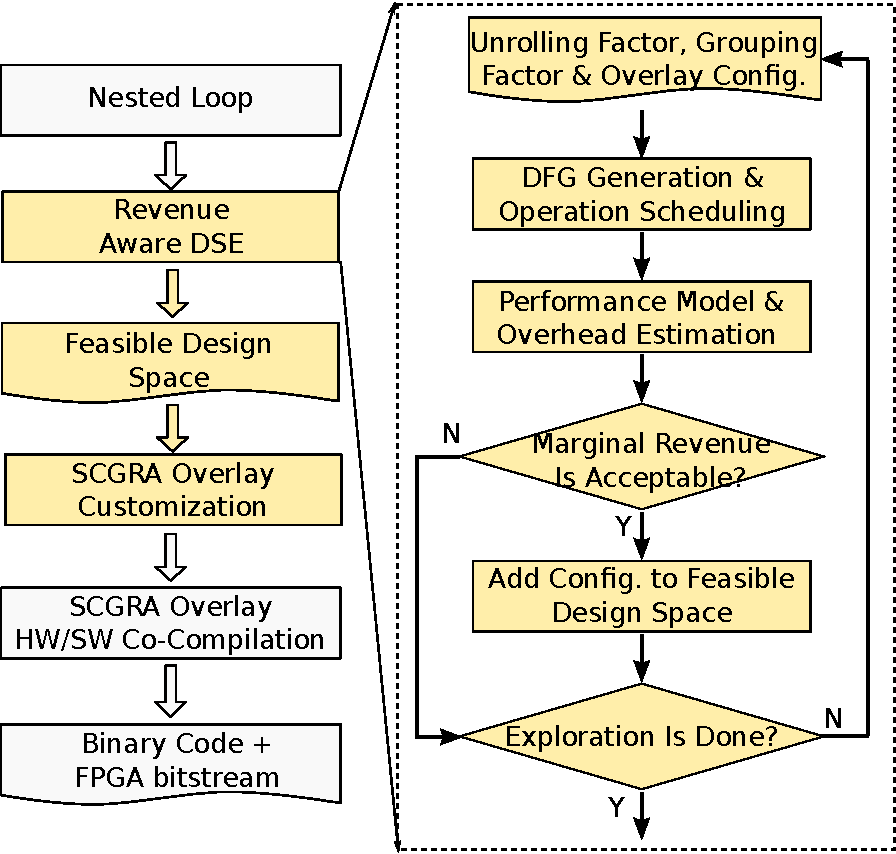
\includegraphics[width=0.8\linewidth]{customization-framework}}
\caption{System customization framework.}
\label{fig:customization-framework}
\end{figure}

Suppose $\Phi$ denotes the feasible design space. $\epsilon$ indicates the
percentage of the performance benefit obtained by the increase 
of loop unrolling or SCGRA size. It is a user defined 
threshold and must be small enough to prune the configurations that are 
inappropriate. The configurations in $\Phi$ must satisfy \eqnref{eq:cond1} 
and \eqnref{eq:cond2}. 
\begin{equation} \label{eq:cond1}
    \scriptsize
    \begin{split}
        &\forall \bm{C}=(...,\bm{u},r,c,...)\in \Phi, \bm{C'}=(...,\bm{u'},r',c',...) \in \Phi,\\ 
        & (r+1==r' \text{ and } c==c') \text{ or } (r==r' \text{ and } c+1==c'): \\ 
        &\frac{CompuTime(\bm{C})-CompuTime(\bm{C'})}{CompuTime(\bm{C})} > \epsilon \\
    \end{split}
\end{equation}

\begin{equation} \label{eq:cond2}
    \scriptsize
    \begin{split}
        &\forall \bm{C}=(...,\bm{u},r,c,...) \in \Phi, \bm{C'}=(...,\bm{u'},r,c,...) \in \Phi,\\ 
        &\bm{u} \text{ and } \bm{u'} \text{ are consecutive unrolling factors}: \\
        &\frac{CompuTime(\bm{C})-CompuTime(\bm{C'})}{CompuTime(\bm{C})} > \epsilon
    \end{split}
\end{equation}

Each configuration $\bm{C} \in \Phi$ must have the corresponding 
scheduling result known, and thus the computation time of the 
loop kernel and minimum instruction memory depth are available as well. Then we can further evaluate 
the performance of each feasible configuration using the models built in 
previous section and obtain the optimized configuration through a simple search.

%In order to achieve the desired customization, we must make sure the 
%FDS acquired from \eqnref{eq:cond1} and \eqnref{eq:cond2} can always 
%cover the configuration that produces the optimal customization. A brief 
%roof is presented as follows.

%$\forall \bm{C'} \notin \Phi$, there must be a configuration $\bm{C}$ that fails 
%\eqnref{eq:cond1} or \eqnref{eq:cond2}. Suppose $\bm{C'}=(...,\bm{u},r+1,c,...)$ 
%and $\bm{C}=(...,\bm{u},r,c,)$. Thus we can conclude that 
%\begin{equation}
%    CompuTime(\bm{C'}) \geq (1-\epsilon) \times CompuTime(\bm{C})
%\end{equation}

%Since $\epsilon$ can be small and unrolling factor is not changed, $DFGCompuTime(\bm{C'})$ 
%roughly equals to $DFGCompuTime(\bm{C})$ and therefore the instruction memory depth 
%will not change. However, the increase of row size of the SCGRA overlay will result in 
%significant overhead of BRAM and power consumption. Thus $Power(\bm{C'}) 
%\geq Power(\bm{C})$. In addition, it will reduce the BRAM budget 
%for on-chip buffer, which means $CommuTime(\bm{C'}) \geq CommuTime(\bm{C})$. 
%According to \eqnref{eq:energy} and \eqnref{eq:runtime}, it is clear 
%that $Energy(\bm{C'}) \geq Energy(\bm{C})$ and 
%any configuration that is pruned during the sub DSE will not be an optimized 
%configuration. Similarly, we can also draw the same conclusion when a different 
%occasion in \eqnref{eq:cond1} and \eqnref{eq:cond2} appears.

In addition, a series of experiments on Zedboard \cite{zedboard} as 
shown in \figref{fig:observation} demonstrate that SCGRA size and 
unrolling factor present a clear monotonic influence on the 
loop compute time. The performance benefit of loop unrolling and 
increase of SCGRA size drops gradually. This observation further helps to simplify the sub DSE with
a simple branch and bound algorithm.

%we can conclude that \eqnref{eq:observation}.
%\begin{equation} \label{eq:observation}
%    \begin{split}
%        CompuTime&(\bm{C_1})-CompuTime(\bm{C_2}) > \\
%                 &CompuTime(\bm{C_2})-CompuTime(\bm{C_3})
%    \end{split}
%\end{equation}
%where $\bm{C_1}=(...,x1,...)$, $\bm{C_2}=(...,x2,...)$, $\bm{C_3}=(...,x3,...)$ and
%$x1$, $x2$, $x3$ are three increasingly consecutive configurations of loop unrolling 
%factor or row or column of the SCGRA overlay.

%In other words, if $\bm{C_1}$ fails to be a feasible configuration, we can be 
%sure that $\bm{C_2}$ and $\bm{C_3}$ will fail as well. With this observation, 
%we can further simplify the sub design space exploration. The simplified sub 
%DSE will be detailed in next section.

\begin{figure}[tb]
    \subfloat[\label{fig:scgrasize-perf}]{%
      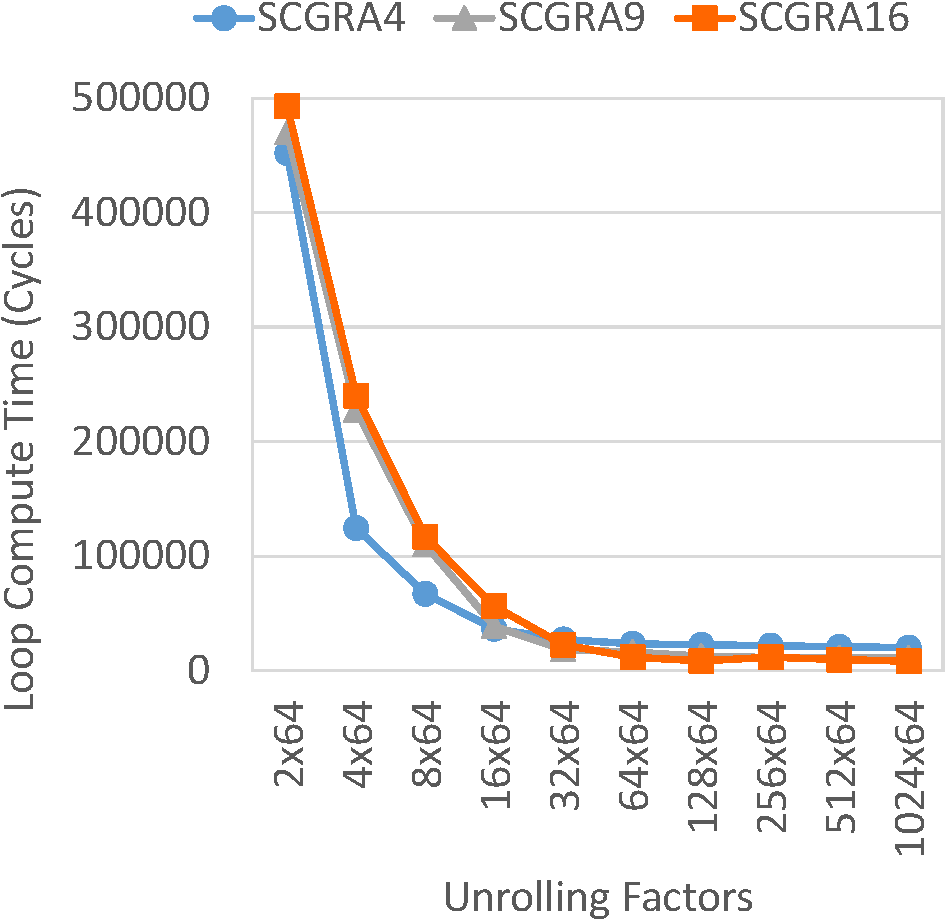
\includegraphics[width=0.235\textwidth]{scgrasize-perf}
    }
    %\hfill
    \subfloat[\label{fig:unrolling-perf}]{%
      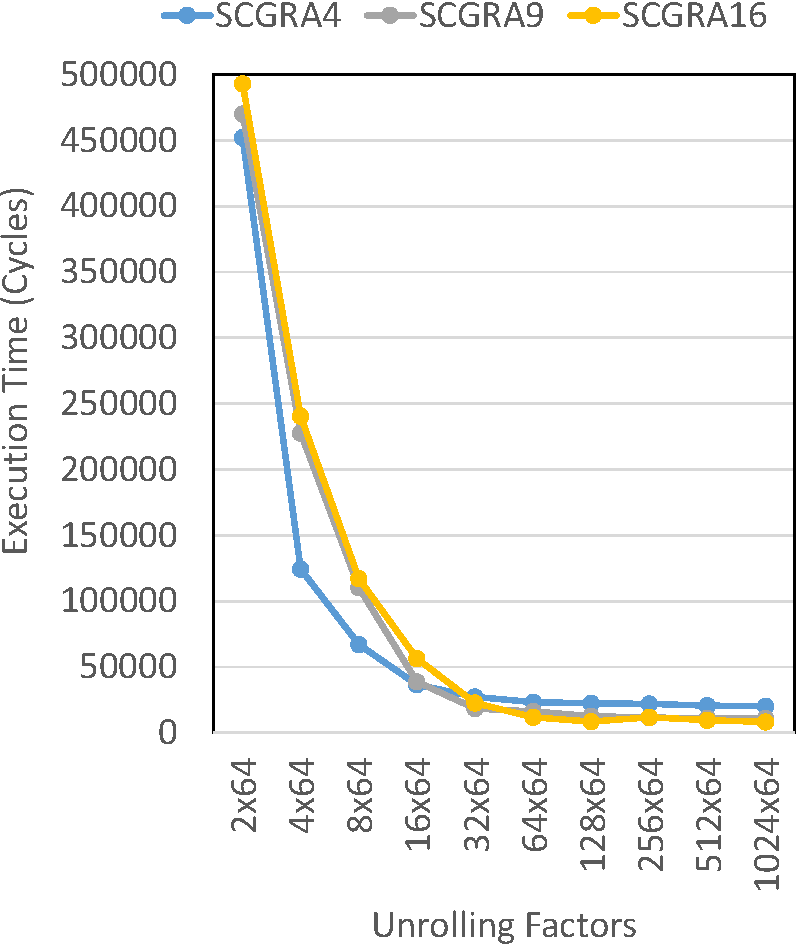
\includegraphics[width=0.22\textwidth]{unrolling-perf}
    }
    \caption{The design parameters typically have monotonic influence on the
        loop computation time and the computation time benefit degrades with 
        the increase of the design parameter. (a) SCGRA Size, (b) Unrolling Factor}
    \label{fig:observation}
  \end{figure}


%\subsection{Sub Design Space Exploration}
%To acquire the FDS, we developed a dedicated sub DSE 
%targeting nested loop computation time. Since the loop computation 
%time merely depends on the SCGRA overlay 
%size and the loop unrolling factor, the sub DSE is much simpler 
%compared to the overall customization problem. In addition, we can 
%further simplify the sub DSE with the observations shown in \figref{fig:observation}.  
%Whenever a configuration fails the sub DSE condition, all the 
%configurations which are larger on one design parameter and remain the same 
%on the rest design parameters can be safely pruned. Thus a branch and 
%bound algorithm as detailed in \algref{alg:revenuealg} is used 
%to efficiently explore the sub design space.
%\begin{algorithm}[h]
%\caption{Sub Design Space Exploration.}
%\label{alg:revenuealg}
%\begin{algorithmic}
%\PROCEDURE{}
%\STATE Initialize $r=2, c=2, \bm{u}=(1,1,...)$, FDS $\Phi=\emptyset$,
%$\bm{C}=(...,r,c,\bm{u},...)$, maximum SCGRA overlay $r_{Max}\times c_{Max}$.
%\WHILE {$r<r_{Max}$} 
%\WHILE {$c<c_{Max}$}
%\WHILE {$\bm{u}$ is not fully unrolled}
%\STATE Generate DFG with $\bm{u}$
%\STATE DFG Scheduling with configuration $\bm{C}$
%\STATE Estimate performance $CompuTime(\bm{C})$
%\STATE Get neighbor $\bm{C'} \in \Phi$ with smaller loop unrolling
%\IF {$\bm{C'}$ exists and $Revenue(\bm{C}, \bm{C'}) \leq \epsilon$}
%\STATE Break
%\ELSE 
%\STATE Add $\bm{C}$ to $\Phi$
%\ENDIF
%\STATE update $\bm{u}$ with larger neighbor unrolling factor
%\ENDWHILE
%\STATE Get neighbor $\bm{C''} \in \Phi$ with smaller column size
%\IF {$\bm{C''}$ exists and $Revenue(\bm{C}, \bm{C''}) \leq \epsilon$}
%\STATE Break
%\ENDIF
%\STATE $c=c+1$
%\ENDWHILE
%\STATE Get neighbor $\bm{C'''} \in \Phi$ with smaller row size
%\IF {$\bm{C'''}$ exists and $Revenue(\bm{C}, \bm{C'''}) \leq \epsilon$}
%\STATE Break
%\ENDIF
%\STATE $r=r+1$
%\ENDWHILE
%\ENDPROCEDURE
%\STATE
%\PROCEDURE {$Revenue(\bm{C}, \bm{C'})$}
%\STATE return $\frac{CompuTime(\bm{C'})-CompuTime(\bm{C})}{CompuTime(\bm{C'})}$ 
%\ENDPROCEDURE
%\end{algorithmic}
%\end{algorithm}
%
%
